\section{Replacing LLVM LLC} \label{sec:llcReplacement}
\textit{LLVM LLC} is a command line tool that takes \textit{LLVM IR} as input and converts it to assembly language for a specified architecture such as \textit{PTX}. Since \textit{LLVM LLC} is a command line tool, it becomes difficult to include this in \textit{YAGAL}, since this would require the library to start, and be dependent upon, an external process. This can be seen on Figure \ref{fig:yagalLLC} where \textit{YAGAL} starts the \textit{LLVM LLC} process and provides it with the \textit{LLVM IR}, and must await the result.

\begin{figure}
    \centering
    \begin{minipage}[t]{0.55\textwidth}\centering%
        \includegraphics[width=\textwidth]{chapters/implementation/figs/LLVMLLC.png}
        \caption{Yagal using LLC.}
        \label{fig:yagalLLC}
    \end{minipage}\hfill
    \begin{minipage}[t]{0.3\textwidth}\centering%
        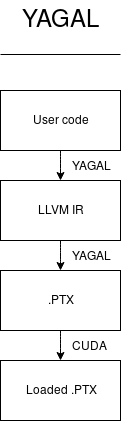
\includegraphics[width=\textwidth - 44pt]{chapters/implementation/figs/YAGALLLC.png} 
        \caption{YAGAL with LLC replacement.}
        \label{fig:noLLC}
    \end{minipage}
\end{figure}

The source code for \textit{LLVM LLC} is open source and available on \textit{GitHub}\cite{llvmGithub}, and we have implemented a subset of it to fit our use case by using the original implementation as an example.

The subset of \textit{LLVM LLC} we implemented involves \textit{PTX} generation as single purpose. It have been implemented directly into \textit{YAGAL} in order to avoid being dependent upon an external processes. This has resulted in the flow which is shown by Figure \ref{fig:noLLC} where the \textit{LLVM LLC} tool is no longer involved in the process.

The \textit{PTX} generation is contained within the \texttt{PTXModule} class. This class functions as a container to generate and hold \textit{PTX} code based on a given \texttt{IRModule}. The constructor of the \texttt{PTXModule} class can be seen in Listing \ref{code:ptxmodule}, and line references in this section is referring to this Listing. 

% Initialize stuff
The \texttt{initializeLlvmTargetIfNeeded} function invokes \textit{LLVM C} macros if they haven not already been invoked. This initializes the \textit{LLVM} backend for \textit{NPTX} which is needed for converting \textit{LLVM IR} to \textit{PTX}. The \texttt{initializeLlvmPassRegistryIfNeeded} function specifies which passes the \textit{NPTX} backend should perform upon the \textit{LLVM IR}.

% Setup - architecture - target machine
At lines \ref{code:ptxmodule:targetVarsBegin} through \ref{code:ptxmodule:targetVarsEnd} we set the variables needed for the target machine. These variables represent options that would have been provided to \textit{LLVM LLC} as command line arguments.

% PassManager
At line \ref{code:ptxmodule:passMan} we initialize the \texttt{PassManager}. A \texttt{PassManager} is an \textit{LLVM} structure that manage the compilation passes. The compilation passes we need are specified in the \texttt{initializeLlvmPassRegistryIfNeeded} function.

% output buffer
% - Siger sig selv

% Machine Module info
A \texttt{LLVMTargetMachine} is instantiated at line \ref{code:ptxmodule:machine} along with a \texttt{MachineModuleInfo} pointer. These contain meta information regarding the target machine which are necessities for LLVM.

% Reset datalayout of module
The data layout for the \texttt{PtxModule} is set at line \ref{code:ptxmodule:layout}. The data layout describes how data is to be laid out in memory. The data layout for the GPU in our test machine is \texttt{e-i64:64-i128:128-v16:16-v32:32-n16:32:64}.

% After data layout
The given passes are registered and initialized by call to the \texttt{addPassesToEmitFile} function at line \ref{code:ptxmodule:emit}. The output buffer is also registered here, which is where we can read the resulting \textit{PTX} code fom.

% pass run & write to string
Finally, the passes are executed at line \ref{code:ptxmodule:runPass}. The result is then witted to a the \texttt{\_string} variable, which is a member of the \texttt{PtxModule} class, at line \ref{code:ptxmodule:writeStr}. The \texttt{\_string} variable is later in the process passed to CUDA through \texttt{yagal::cuda::cudaHandler} for execution.

\begin{lstlisting} [caption={\texttt{PTXModule} constructor based on a given \texttt{IRModule}.}, label={code:ptxmodule}]
PTXModule(IRModule& ir){
    initializeLlvmTargetIfNeeded();
    initializeLlvmPassRegistryIfNeeded();

    std::string arch("nvptx64"); ~\label{code:ptxmodule:targetVarsBegin}~
    llvm::Triple triple(llvm::Twine("nvptx64-nvidia-cuda"));
    std::string error;
    const llvm::Target *target(
        llvm::TargetRegistry::lookupTarget(
            arch, triple, error));
    std::string cpuStr("sm_20");
    std::string featureStr("");
    llvm::CodeGenOpt::Level optLevel(
        llvm::CodeGenOpt::Aggressive);
    llvm::TargetOptions options;~\label{code:ptxmodule:targetVarsEnd}~

    std::unique_ptr<llvm::TargetMachine> ~\label{code:ptxmodule:targetMachine}~
        targetMachine(target->createTargetMachine(
        triple.getTriple(), 
        cpuStr, 
        featureStr, 
        options, 
        llvm::None, 
        llvm::CodeModel::Small, 
        optLevel));

    llvm::legacy::PassManager passManager; ~\label{code:ptxmodule:passMan}~

    llvm::SmallVector<char, 512> buffer; ~\label{code:ptxmodule:buffer}~
    auto bufferStream = 
        std::make_unique<llvm::raw_svector_ostream>(buffer);
    auto outputStream = bufferStream.get();

    llvm::LLVMTargetMachine &llvmtm = ~\label{code:ptxmodule:machine}~
        static_cast<llvm::LLVMTargetMachine&>(*targetMachine);
    llvm::MachineModuleInfo *mmi = 
        new llvm::MachineModuleInfo(&llvmtm);

    ir.module.setDataLayout( ~\label{code:ptxmodule:layout}~
        targetMachine->createDataLayout());
    targetMachine->addPassesToEmitFile( ~\label{code:ptxmodule:emit}~
        passManager, *outputStream, 
        llvm::TargetMachine::CGFT_AssemblyFile, false, mmi);

    passManager.run(ir.module); ~\label{code:ptxmodule:runPass}~

    _string = std::string(buffer.begin(), buffer.end()); ~\label{code:ptxmodule:writeStr}~

    _p.debug() << "ptx module constructed" << std::endl;
}
\end{lstlisting}